We know that in special relativity we must have our velocities sum in such a way that the velocity of light will not change, but the velocity of slower objects will (and in the non-relativistic limit they simply add).
We can say:
\begin{align*}
	dt' &= \gamma(dt - vdx) \\
	dx' &= \gamma(dx -v dt) \\
	\frac{dx'}{dt'} &= \frac{\frac{dx}{dt} - v}{1 -v \frac{dx}{dt}}
\end{align*}
If we choose $\frac{dx}{dt} = 1$ then $\frac{dx'}{dt'} = 1$. So this works for light like velocities how we want it to.

\subsection{Four vectors and coordinate systems}
We can write our line element in terms of our metric:
\begin{align*}
	ds^2 &= \eta_{\alpha\beta} dx^\alpha dx^\beta
\end{align*}
We tend to paramterize paths in terms of the proper time of the particle while moving. So our four velocity in terms of the proper time is then:
\begin{align*}
	u^\alpha &= \frac{dx^\alpha}{d\tau}
\end{align*}
Our temporal component is then going to be $u^t = \gamma$ and our spatial components are $u^i = \gamma v^i$, so we cam say our four velocity is then $u^\mu = (\gamma,\gamma \bm{V}$
\subsection{Dynamics}
We now consider Newton's first law in special relativity:
\begin{align*}
	\frac{d u^\mu}{d\tau} &= 0
\end{align*}
In the abscence of forces. In order to posit Newton's second law, we want it to abey this in the abscence of forces, be properly relativistic, and reduce to the classical result in the non-relativistic limit:
\begin{align*}
	m\frac{du^\mu}{d\tau} &= f^\mu
\end{align*}
Which since this is a 4-vector equation obviously obeys relativity, and it clearly obeys the first law when $f^\mu =0$. In order to check the classical limit, we define the four acceloration $a^\mu = \frac{du^\mu}{d\tau}$.
This gives us the classic $f^\mu = m a^\mu$. This is a set of 4 equations, which is one more than our classical set of equations. This is of course constrained by our restriction on the length of $u$, $u^\mu u_\mu = -1$, so:
\begin{align*}
	m \frac{d}{d\tau} u^\mu u_\mu &= 0 \\
	u^\mu a_\mu &= 0 \\
	f_\mu u^\mu &=0
\end{align*}
We now look at energy and momentum.
\begin{align*}
	p^\mu &= m u^\mu \\
	\frac{dp^\mu}{d\tau} &= f^\mu \\p^\mu p_\mu &= -m^2 \\
	p^t &= \frac{m}{1-v^2} \\
	p^i &= \frac{mv^i}{\sqrt{1-v^2}}
\end{align*}
If we take the limit where $v\ll 1$:
\begin{align*}
	p^t &= m + \frac{1}{2} mv^2 \\
	p^i &= mv^i
\end{align*}
So we say $p^\mu = (E, P)$

We now look to extract our spatial forces from our 4 force. We define this by $F^i = \frac{dP^i}{dt}$, so:
\begin{align*}
	f^i &= \frac{dP^i}{d\tau} \\
	f^i &= \gamma F^i
\end{align*}
We also know:
\begin{align*}
	f^t u^t &= f_i u^i \\
	f_t\gamma &= \gamma^2 F_i V^i \\
	f^t &= \gamma F_i V^i \\
	f^\mu &= (\gamma F_i V^i, \gamma F^i)
\end{align*}
\section{Curved Spacetime}
We say that our line element:
\begin{align*}
	ds^2 &= -dt^2 + dx^2 + dy^2 + dz^2
\end{align*}
Can be used to find line elements in other coordinate systems, such as with spherical coordinates. Here we will have:
\begin{align*}
	ds^2 &= -dt^2 + dr^2 + r^2 d\theta^2 + r^2\sin^2\theta d\phi^2
\end{align*}
This introduces a coordinate singularity, as if you choose $\theta=0$ all values for $\phi$ are mapped to the same point. This is non-physical though as it doesn't appear in caresian coordinates.

Let us now consider 2-D polar coordinates in flat space:
\begin{align*}
	dS^2 &= dr^2 = r^2d\phi^2
\end{align*}
If we transform to $r = \frac{a^2}{r'}$:
\begin{align*}
	dS^2 &= \frac{a^4}{r'\ ^4} (dr'\ ^2 + r'\ ^2 d\phi^2)
\end{align*}
Which has an infinite line element at $r' = 0$, but this makes sense as our transformation only gives us $r' = 0$ if $r = \infty$.
\subsection{Penrose diagrams}
We begin with our line element for flat spacetime in spherical coordinates:
\begin{align*}
	ds^2 &= -dt^2 + dr^2 + r^2 d\theta^2 + r^2\sin^2\theta d\phi^2
\end{align*}
We now define a coordinate $u = t - r$ and $v = t + r$, then we see we have a new line element:
\begin{align*}
	ds^2 &= -dudv + \frac{1}{4} (u-v)^2 (d\theta^2 \sin^2\theta d\phi^2)
\end{align*}
This implies off diagonal metric elements. In this coordinate system, lines of constant $u$ and $v$ are light paths.

We now make one more transformation:
\begin{align*}
	u' &= \arctan u &
	u' &= \frac{t' - r'}{2} \\
	v' &= \arctan{v} &
	v' &= \frac{t' + r'}{2}
\end{align*}
This will map all $(t,r)$ to $r' > 0$, $v' < \frac{\pi}{2}$, $u' > -\frac{\pi}{2}$
\begin{figure*}[h]
	\centering
	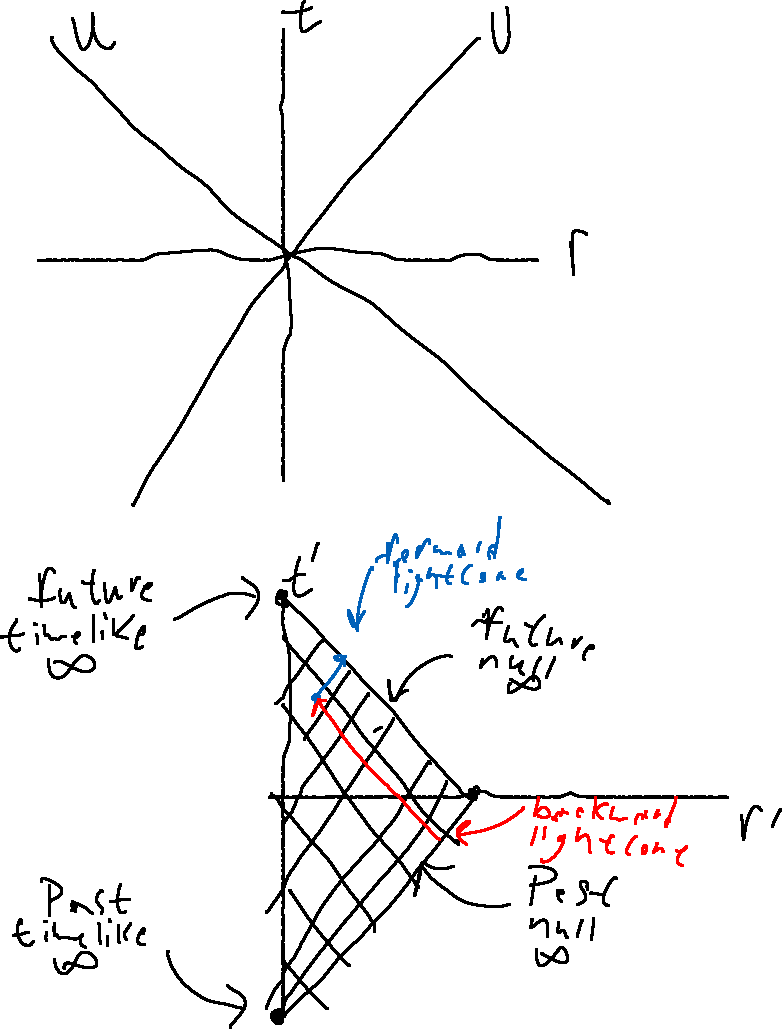
\includegraphics[width=6cm]{1-14-1.png}
	\caption*{Penrose Diagrams}
\end{figure*}
\subsection{Local Inertial frames}
We say that the equivalence priciple states that in local coordinates it is impossible to determine whether or not you are in curved spacetime.

In general we refer to our metric as $g_{\alpha\beta}$. Given some general metric (as a function of spacetime) $g_{\alpha\beta}(\bm{x})$, at every point $P$ we can invent a new coordinate system where:
\begin{align*}
	g_{\alpha\beta}'(x'_P) &= \eta_{\alpha\beta} \\
	\partder{g_{\alpha\beta}}{x'}|_P &= 0
\end{align*}
Which defines a local inertial frame at $p$.

Just as before we have the following types of distance:
\begin{align*}
	ds^2 < 0 & \text{timelike} \\
	ds^2 &= 0 & \text{null/lightlike} \\
	ds^2 >0 & \text{spacelike}
\end{align*}
Where our proper time can be defined as:
\begin{align*}
	\tau_{AB} &= \int_A^B \sqrt{-g_{\alpha\beta}(x)dx^\alpha dx^\beta}
\end{align*}
\subsection{Length, area, volume, and 4-volume}
For now we consider:
\begin{align*}
	ds^2 &= g_{00} (dx^0)^2 + g_{11}(dx^1)^2 + g_{22} (dx^2)^2 + g_33(dx^3)^2
\end{align*}
Therefore our area can be expressed as (for a rectangle in $x^1$, $x^2$):
\begin{align*}
	dA &= \sqrt{g_{11} g_{22}} dx^1 dx^2
\end{align*}
And for our three volume:
\begin{align*}
	dV &= \sqrt{g_{11}g_{22}g_{33}} dx^1 dx^2 dx^3 
\end{align*}
and finally four volume:
\begin{align*}
	dv &= \sqrt{-g_{00}g_{11}g_{22} g_{33}}dx^0dx^1dx^2dx^3
\end{align*}
If we let $g$ denote $\det g_{\alpha\beta}$ then:
\begin{align*}
	dv &= \sqrt{g} d^4 x
\end{align*}

We now consider the line element:
\begin{align*}
	dS^2 &= \frac{dr^2}{1-\left(\frac{r}{a}\right)^2} + r^2(d\theta^2 + \sin^2\theta d\phi^2)
\end{align*}
If we look at $r=R$ and $\theta = \frac{\pi}{2}$ then we calculate our circuference:
\begin{align*}
	C &= \oint dS \\
	C &= 2\pi R
\end{align*}
And then the distance from the center to the surface alone a line of constant $\theta$ and $\phi$:
\begin{align*}
	S &= \int dS \\
	S &= a\arcsin \frac{R}{a}
\end{align*}
Looking at the area of our surface at constant radius we find:
\begin{align*}
	A &= \int dA \\
	A &= 4\pi R^2
\end{align*}
And we finally consider the volume inside a radius $R$:
\begin{align*}
	V &= \int dV \\
	V &= \int_0^R dr\in_0^\pi d\theta\int_0^{2\pi}d\phi \frac{r^2\sin\theta}{1-\left(\frac{r}{a}\right)^2} \\
	V &= 4\pi a^3 \left(\frac{1}{2}\arcsin\left[\frac{R}{a}  - \frac{R}{2a} \sqrt{1 - \left(\frac{R}{a}\right)^2}\right]\right)
\end{align*}

\subsection{Embedding Diagrams}
We consider the line element:
\begin{align*}
	ds^2 &= -dt^2 + dr^2 +(b^2 + r^2)(d\theta^2 + \sin^2\theta d\phi^2)
\end{align*}
(Note we call this a static metric since there is no explicit time dependance). This is flat when $b=0$ but is not flat otherwise.

We now consider a slice where $t$ is constant:
\begin{align*}
	dS^2 &= dr^2 +(b^2 + r^2)(d\theta^2 + \sin^2\theta d\phi^2)
\end{align*}
And now constant angle ($\theta = \frac{\pi}{2}$:
\begin{align*}
	d\Sigma^2 &= dr^2 +(b^2 + r^2)d\phi^2
\end{align*}
We now consider this in cylindrical coordinates in flat space:
\begin{align*}
	dS^2 &= d\rho^2 + \rho^2 d\psi^2 + dz^2
\end{align*}
We look at this in terms of $z= z(r)$, $\rho = \rho(r)$ and $\psi = \phi$
We then have:
\begin{align*}
	d\psi &= d\phi \\
	dz &= \frac{dz}{dr} dr \\
	d\rho &= \frac{d\rho}{dr} dr
\end{align*}
So then:
\begin{align*}
	d\Sigma^2 &= \left(\frac{d\rho}{dr}\right)^2 dr^2 + \rho^2d\phi^2 + \left(\frac{dz}{dr}\right)^2 dr^2 \\
	d\Sigma^2 &= \left[\left(\frac{d\rho}{dr}\right)^2+ \left(\frac{dz}{dr}\right)^2 \right] dr^2 + \rho^2d\phi^2
\end{align*}
So then by inspection:
\begin{align*}
	\rho^2 &= r^2 + b^2 \\
	\left(\frac{dz}{dr}\right)^2 + \left(\frac{d\rho}{dr}\right)^2 &= 1 \\
	\left(\frac{d\rho}{dr}\right)^2 &= \frac{r^2}{\rho^2} \\
	\left(\frac{d\rho}{dr}\right)^2 &= \frac{r^2}{r^2 + b^2} \\
	\left(\frac{dz}{dr}\right)^2 &= \frac{1}{1 + \left(\frac{r}{b}\right)^2} \\
	z &= b\text{arcsinh}\frac{r}{b}
\end{align*}
